\documentclass[conference]{IEEEtran}

\usepackage{amsmath}
\usepackage{amssymb}
\usepackage{algorithm}
\usepackage{algpseudocode}
\usepackage{booktabs}
\usepackage{array}
\usepackage{graphicx}
\usepackage{multirow}
\usepackage{svg}
\usepackage{url}

\title{A Multi-Strategy Self-Healing Software-Defined Network with Telemetry, Adaptive Control, and Recovery Evidence}

\author{\IEEEauthorblockN{Student Research Project}
\IEEEauthorblockA{Department of Computer Science\\
SDN and Network Automation Laboratory}}

\begin{document}
\maketitle

\begin{abstract}
Network failures, congestion, delay, and packet loss can interrupt services
even when alternate routes exist. This paper presents a complete self-healing
software-defined networking platform implemented with Mininet, Open vSwitch,
Ryu, OpenFlow 1.3, NetworkX, FastAPI, SQLite, and React. The system combines
four controller strategies---baseline shortest-path forwarding, reactive
flow-repair, OpenFlow fast failover, and adaptive policy control---with two
redundant network topologies. A telemetry subsystem derives rates,
utilization, packet drops, and errors from OpenFlow counters. A rule-based
alert subsystem detects congestion and abnormal host traffic, while a
labelled-data workflow records latency, jitter, and end-to-end loss under
controlled scenarios. The management layer persists experiments and events in
SQLite and exposes health, topology, telemetry, alert, and experiment APIs.
The React dashboard presents operational state, measurements, and experiment
history. Mathematical models for path selection, utilization, loss, alert
thresholds, and recovery scoring are defined. Results from the labelled
traffic data show average RTT values of 26.80 ms for idle traffic, 30.98 ms
under 2 Mbps load, 70.83 ms under 4 Mbps load, and 157.00 ms during delay
ramp. The complete design provides an extensible research platform for
measurable SDN resilience and automated recovery.
\end{abstract}

\begin{IEEEkeywords}
software-defined networking, self-healing networks, OpenFlow, Mininet, Ryu,
fast failover, network telemetry, network recovery
\end{IEEEkeywords}

\section{Introduction}
\label{sec:introduction}

Modern networked services depend on continuous reachability and predictable
latency. A single physical or logical link failure can interrupt a service even
when the topology contains a redundant path. Manual diagnosis and repair
introduce delay, require operator intervention, and provide limited quantitative
evidence about the recovery process. Soft degradation is equally important:
increased delay, packet loss, or link utilization can violate a service
objective while the interface remains operational.

Software-defined networking (SDN) separates forwarding decisions from the
data plane and exposes programmable control through OpenFlow. A controller can
maintain a topology graph, calculate a path, install forwarding rules, receive
link-status events, and select an alternate route. OpenFlow fast-failover
groups extend this model by allowing the switch to select a backup bucket
using local port state. These mechanisms provide complementary trade-offs:
controller-driven recovery is flexible and observable, while switch-local
failover can reduce dependence on a controller round trip.

This project develops a complete self-healing SDN platform around a small
four-switch diamond topology and a larger multipath mesh. The first layer is a
Ryu/Mininet prototype that demonstrates shortest-path forwarding, link-failure
detection, port telemetry, threshold-based alerting, and labelled traffic
data. The expanded layer adds reusable controller strategies, dynamic
topology discovery, a multipath topology, a FastAPI management service, SQLite
history, a React dashboard, and a structured research-report workflow.

The main contributions are:
\begin{itemize}
\item a graph-based routing and recovery model for redundant SDN topologies;
\item four comparable controller strategies with distinct failure behavior;
\item reactive flow deletion and reinstallation after a failed link;
\item OpenFlow fast-failover groups with watch-port buckets;
\item OpenFlow port-counter telemetry and threshold-based alert generation;
\item labelled latency, jitter, and loss data for service-level analysis;
\item a management API, persistent experiment records, and dashboard view;
\item a measurement model that separates configuration, controller events,
  service observations, and dataplane evidence.
\end{itemize}

\section{Related Work}
\label{sec:related}

OpenFlow introduced a programmable interface between a control application and
switch forwarding tables, enabling experimentation with network policy and
path control \cite{mckeown2008}. The OpenFlow 1.3 specification provides flow
modification messages, port-status events, and group tables used by the
controllers in this project \cite{openflow13}. Ryu supplies an event-driven
Python framework for receiving these events and constructing OpenFlow
messages \cite{ryu}.

Mininet provides lightweight virtual hosts, switches, and links in a single
Linux environment, making it suitable for repeatable SDN experiments
\cite{lantz2010}. NetworkX supplies graph algorithms used here for shortest
paths and distance-based backup-port selection \cite{networkx}. Existing SDN
resilience approaches generally fall into controller-rerouting, proactive
backup installation, or local protection categories. The present system
implements representatives of all three: the baseline and reactive
controllers calculate routes, the fast-failover controller proactively
installs backup buckets, and the adaptive controller provides a policy
boundary for selecting bounded recovery actions.

The project also connects forwarding recovery with observability. Rather than
measuring only whether a flow rule was sent, the system records OpenFlow
counters, utilization, packet loss, RTT, jitter, alerts, and experiment
metadata. This makes it possible to distinguish a controller event from an
actual service result.

\section{Problem Scenario}
\label{sec:problem}

The primary scenario is an edge-to-edge service between hosts connected
through redundant switches. In the diamond topology, host $h_1$ connects to
$s_1$ and host $h_4$ connects to $s_4$. There are two switch-level routes:
\begin{align}
 P_{\mathrm{primary}} &= h_1\rightarrow s_1\rightarrow s_2
 \rightarrow s_4\rightarrow h_4,\\
 P_{\mathrm{backup}} &= h_1\rightarrow s_1\rightarrow s_3
 \rightarrow s_4\rightarrow h_4.
\end{align}
The primary route has lower configured cost. When a link on that route fails,
the controller must remove the failed edge from its graph, select a valid
backup, and update forwarding rules. When a link remains operational but
experiences delay or loss, the health subsystem must report degradation
without confusing a soft condition with a hard port-down event.

\subsection{Failure classes}

The system models three operational classes:
\begin{enumerate}
\item \textit{Hard failure}: an OpenFlow port-status or topology event marks
  an inter-switch link unavailable.
\item \textit{Soft degradation}: delay, packet loss, or utilization increases
  while the interface remains operational.
\item \textit{Service impact}: end-to-end packet loss, RTT, or jitter changes
  as observed by traffic or ping accounting.
\end{enumerate}
These classes are intentionally separate. A configured delay is not an RTT
measurement, and a controller processing interval is not the duration of a
service outage.

\subsection{Research questions}

The project evaluates the following questions:
\begin{enumerate}
\item Can graph-based forwarding maintain connectivity across a redundant
  topology after a hard link failure?
\item How do reactive and fast-failover mechanisms differ in control behavior?
\item Can OpenFlow counter telemetry identify utilization and traffic anomalies?
\item How does delay or load affect end-to-end RTT and jitter?
\item Can a management layer preserve experiment identity, history, and
  measurement context across controller strategies?
\end{enumerate}

\section{System Model}
\label{sec:system}

\subsection{Network graph}

The switch fabric is represented by an undirected graph
$G=(V,E,w)$, where $V$ is the switch set, $E$ is the inter-switch link set,
and $w:E\rightarrow\mathbb{R}^{+}$ assigns a route cost. Host attachment
points are represented as tuples $(d,p)$ containing a switch datapath identifier
$d$ and an output port $p$. The original topology has four switches and two
hosts. The mesh extension has nine switches, two hosts, and twelve
inter-switch links with multiple redundant routes.

\begin{table}[t]
\centering
\caption{Network topologies}
\label{tab:topologies}
\begin{tabular}{lccc}
\toprule
Topology & Switches & Hosts & Internal links\\
\midrule
Diamond & 4 & 2 & 4\\
Multipath mesh & 9 & 2 & 12\\
\bottomrule
\end{tabular}
\end{table}

\subsection{Software architecture}

The architecture is divided into five layers:
\begin{enumerate}
\item \textit{Data plane}: Mininet hosts, Open vSwitch bridges, TCLinks, and
  OpenFlow 1.3 switch tables.
\item \textit{Controller plane}: Ryu applications implementing baseline,
  reactive, fast-failover, and adaptive modes.
\item \textit{Observation plane}: port-statistics polling, CSV telemetry,
  traffic results, alerts, and recovery records.
\item \textit{Management plane}: FastAPI endpoints, SQLite persistence,
  topology catalog, experiment records, and event history.
\item \textit{Presentation plane}: React/Vite dashboard for health, telemetry,
  topology catalog, and experiment history.
\end{enumerate}

\subsection{Telemetry model}

The telemetry controller polls each connected datapath once per second. For
each port it stores the previous timestamp and OpenFlow counters, then derives
transmit and receive rates, packets per second, utilization, drops, and
errors. The records are written to \texttt{data/telemetry.csv}. The management
API reads the latest bounded window and returns both rows and a summary.

\subsection{Management model}

The FastAPI application initializes three SQLite tables: \texttt{experiments},
\texttt{events}, and \texttt{recovery\_records}. The API provides:
\begin{itemize}
\item \texttt{/api/health} for service and telemetry status;
\item \texttt{/api/topologies} and \texttt{/api/topology/\{name\}};
\item \texttt{/api/telemetry} for rows and utilization summaries;
\item \texttt{/api/alerts} and \texttt{/api/events};
\item \texttt{/api/experiments} for experiment planning and history.
\end{itemize}
The dashboard calls these endpoints through a Vite development proxy and
renders health, telemetry, topology count, and experiment history.

\section{Mathematical Formulation}
\label{sec:math}

\subsection{Shortest-path objective}

For source switch $s$ and destination switch $d$, the selected path is:
\begin{equation}
 P^{*}(s,d)=\arg\min_{P\in\mathcal{P}(s,d)}
 \sum_{e\in P}w(e),
\label{eq:shortest}
\end{equation}
where $\mathcal{P}(s,d)$ is the set of available paths. On a failure, the
failed edge is removed from $E$ and the objective is recomputed over
$G'=(V,E\setminus\{e_f\})$.

\subsection{Path validity}

A candidate path is valid when every consecutive pair is an available edge:
\begin{equation}
 \mathrm{valid}(P,G)=
 \prod_{i=0}^{|P|-2}\mathbf{1}
 \left[(P_i,P_{i+1})\in E\right].
\label{eq:valid}
\end{equation}
The reactive controller selects the minimum-cost valid path. The fast-failover
controller selects a next-hop port from neighbors whose distance to the
destination is strictly smaller than the current switch distance. This
monotonic-distance rule prevents forwarding loops.

\subsection{Counter rates}

Let $C_t$ denote a byte counter, $N_t$ a packet counter, and
$\Delta t=t-t_0$. The rates are:
\begin{align}
 r_{\mathrm{Mbps}} &= \frac{8(C_t-C_{t_0})}{10^6\Delta t},\\
 r_{\mathrm{pps}} &= \frac{N_t-N_{t_0}}{\Delta t}.
\label{eq:rates}
\end{align}
For configured link capacity $B$, utilization is:
\begin{equation}
 U=100\frac{\max(r_{\mathrm{tx}},r_{\mathrm{rx}})}{B}.
\label{eq:utilization}
\end{equation}
The prototype uses $B=10$ Mbps for switch-to-switch links.

\subsection{Congestion and anomaly detection}

The congestion detector maintains a three-sample link window:
\begin{equation}
 \overline{U}_3(t)=\frac{U(t)+U(t-1)+U(t-2)}{3}.
\end{equation}
It raises a congestion alert when $\overline{U}_3(t)\geq55\%$. Host
traffic uses a 15-sample warm-up and an exponentially updated baseline:
\begin{equation}
 B_t=0.9B_{t-1}+0.1r_t.
\end{equation}
An anomaly is emitted when:
\begin{equation}
 r_t>2\ \mathrm{Mbps}
 \quad\land\quad r_t>5\max(B_t,0.1).
\label{eq:anomaly}
\end{equation}
A ten-second cooldown limits repeated alerts for the same source or link.

\subsection{End-to-end service loss}

For a traffic window with $T_x$ transmitted and $R_x$ received packets:
\begin{equation}
 L_{\mathrm{e2e}}=100\frac{T_x-R_x}{T_x},\quad T_x>0.
\label{eq:loss}
\end{equation}
Average RTT and jitter are calculated from the received-packet sample set.
These metrics measure service behavior between hosts and are distinct from a
link's configured impairment.

\subsection{Recovery quality score}

For a recovery observation, the project uses a normalized score to support
comparison:
\begin{equation}
 Q=\alpha R+\beta(1-L_n)+\gamma(1-D_n)
\end{equation}
where $R\in\{0,1\}$ is reachability, $L_n$ is normalized loss,
$D_n$ is normalized delay, and $\alpha+\beta+\gamma=1$. A course experiment
can set $\alpha=0.5$, $\beta=0.3$, and $\gamma=0.2$ to prioritize reachability.

\section{Proposed Algorithm and Methodology}
\label{sec:method}

\subsection{Controller initialization}

Each controller records connected datapaths, installs a priority-zero
controller rule, discovers switches and links through Ryu topology events, and
learns host locations from packet-in frames. Inter-switch ports are separated
from host-facing ports using the discovered link inventory.

\begin{algorithm}
\caption{Topology discovery and forwarding setup}
\label{alg:setup}
\begin{algorithmic}[1]
\Require Ryu datapath events and topology events
\ForAll{switch feature messages}
  \State store datapath identifier and parser
  \State install priority-zero controller rule
\EndFor
\ForAll{topology updates}
  \State clear graph, link-port map, and inter-switch port set
  \State add discovered switches to $V$
  \State add discovered links to $E$ with both endpoint ports
\EndFor
\ForAll{packet-in frames}
  \State learn source MAC location on host-facing ingress ports
  \State flood unknown destinations only to edge ports
  \State calculate and install destination forwarding state
\EndFor
\end{algorithmic}
\end{algorithm}

\subsection{Baseline strategy}

The baseline controller provides a comparison reference. It discovers the
topology, learns hosts, calculates a shortest path for known destinations, and
installs ordinary output actions. When a link-delete event is received, it
rebuilds the graph and logs the event without invoking an automatic repair
procedure. This gives experiments a forwarding strategy without self-healing.

\subsection{Reactive strategy}

The reactive controller stores installed paths by destination MAC. When a link
is deleted, it identifies every stored path containing that link, deletes the
destination flows on the affected path, calculates a new shortest path, and
installs fresh output rules. It records the previous path, replacement path,
and controller processing interval.

\begin{algorithm}
\caption{Reactive link-failure recovery}
\label{alg:reactive}
\begin{algorithmic}[1]
\Require graph $G$, installed path set $\Pi$, failed link $(a,b)$
\State $t_0\gets\mathrm{monotonic\_clock}()$
\State remove $(a,b)$ from $G$
\ForAll{$(m,P)\in\Pi$ where $(a,b)\in P$}
  \State delete all flows matching destination $m$ on $P$
  \State $P'\gets\mathrm{shortest\_path}(G,P_0,\mathrm{dst}(m))$
  \If{$P'$ exists}
    \State install output rules for $P'$
    \State replace $P$ with $P'$ in $\Pi$
    \State log $P\rightarrow P'$ and elapsed processing time
  \Else
    \State log destination $m$ as unreachable
  \EndIf
\EndFor
\end{algorithmic}
\end{algorithm}

\subsection{Fast-failover strategy}

The fast-failover controller associates a group identifier with each learned
destination. For every switch, it finds neighbors closer to the destination
than the current switch. It creates an OpenFlow type-FF group with one bucket
per candidate port. Each bucket watches its output port and emits the packet
through that port when selected. The destination flow action is
\texttt{group(group\_id)} rather than a single output action.

\begin{algorithm}
\caption{Fast-failover group installation}
\label{alg:ff}
\begin{algorithmic}[1]
\Require graph $G$, destination switch $d$, destination port $p_d$
\State $dist\gets\mathrm{BFS\_distances}(G,d)$
\ForAll{switches $v\in V$}
  \If{$v=d$}
    \State install output action $p_d$
  \Else
    \State $C_v\gets\{u\in N(v):dist(u)<dist(v)\}$
    \State $P_v\gets$ ports from $v$ to each $u\in C_v$
    \State create FF buckets with $watch\_port=P_v$
    \State install destination flow with group action
  \EndIf
\EndFor
\end{algorithmic}
\end{algorithm}

\subsection{Adaptive strategy}

The adaptive controller shares topology discovery and initial forwarding with
the baseline strategy. Its link-delete handler records the incident and leaves
the recovery decision to the backend policy layer. The policy boundary accepts
telemetry and service measurements, evaluates candidate actions, and bounds
recovery attempts. This design allows additional policies without changing
the OpenFlow controller contract.

\subsection{Telemetry methodology}

The telemetry application keeps a previous counter snapshot for every
$(switch,port)$ pair. It ignores the reserved local port, computes deltas,
maps inter-switch ports to link labels, and flushes every CSV row. The alert
follower starts at the end of the file, parses new rows, maintains utilization
windows and host baselines, and writes timestamped alert blocks.

\subsection{Experiment methodology}

An experiment consists of:
\begin{enumerate}
\item selecting controller and topology;
\item starting the Ryu process and Mininet data plane;
\item confirming switch and link discovery;
\item generating a controlled ICMP or iperf3 traffic window;
\item injecting a hard failure or soft degradation;
\item recording controller events, telemetry, alerts, and service counters;
\item restoring the network and storing the experiment summary.
\end{enumerate}
The FastAPI service assigns an experiment identifier and persists its
configuration. The dashboard reads current telemetry and experiment history,
which provides a single view of the control and observation planes.

\section{Baseline Algorithms and Experimental Setup}
\label{sec:setup}

\subsection{Controller comparison}

\begin{table}[t]
\centering
\caption{Controller strategies and measured behavior}
\label{tab:controllers}
\begin{tabular}{p{0.18\columnwidth}p{0.34\columnwidth}p{0.30\columnwidth}}
\toprule
Strategy & Forwarding mechanism & Recovery behavior\\
\midrule
Baseline & Shortest path and output flow & Logs failure and rebuilds topology\\
Reactive & Shortest path and destination flows & Deletes affected flows and installs a new path\\
Fast failover & Type-FF group with watch ports & Switch selects an operational bucket\\
Adaptive & Initial forwarding plus policy boundary & Backend evaluates bounded recovery actions\\
\bottomrule
\end{tabular}
\end{table}

\subsection{Hardware and software configuration}

\begin{table}[t]
\centering
\caption{Experimental configuration}
\label{tab:configuration}
\begin{tabular}{ll}
\toprule
Component & Configuration\\
\midrule
Virtual network & Mininet with Open vSwitch\\
Control protocol & OpenFlow 1.3\\
Controller framework & Ryu\\
Graph library & NetworkX\\
Switch-link capacity & 10 Mbps\\
Base switch-link delay & 5 ms\\
Telemetry interval & 1 s\\
Congestion threshold & 55\% three-sample average\\
Anomaly warm-up & 15 samples\\
Anomaly threshold & 2 Mbps and $5\times$ baseline\\
Backend & FastAPI and SQLite\\
Frontend & React, TypeScript, Vite\\
\bottomrule
\end{tabular}
\end{table}

\subsection{Traffic scenarios}

The labelled-data workflow uses five-packet ping samples and records
\texttt{timestamp}, \texttt{scenario}, \texttt{label}, \texttt{rtt\_ms},
\texttt{jitter\_ms}, and \texttt{loss\_pct}. The scenarios are:
\begin{itemize}
\item \textit{idle}: no additional load;
\item \textit{load\_2M}: approximately 2 Mbps background load;
\item \textit{load\_4M}: approximately 4 Mbps background load;
\item \textit{delay\_ramp}: progressively increased link delay;
\item \textit{loss\_ramp} and \textit{congestion}: configured degradation cases.
\end{itemize}

\subsection{Data processing}

The stored data is grouped by scenario. For each group, sample count,
arithmetic mean RTT, arithmetic mean jitter, and arithmetic mean loss are
reported. The results graph uses the scenario mean RTT and annotates the sample
count. Alert results are summarized from the timestamped alert log. No values
are extrapolated across scenarios.

\section{Results}
\label{sec:results}

\subsection{Labelled traffic results}

Table~\ref{tab:labelled} summarizes the labelled traffic data. Increasing load
and delay produce a clear increase in average RTT. The 4 Mbps case also has a
small nonzero average packet loss, showing that service quality can change
before a hard link-down event.

\begin{table}[t]
\centering
\caption{Labelled traffic measurements}
\label{tab:labelled}
\begin{tabular}{lrrrr}
\toprule
Scenario & Samples & Avg. RTT (ms) & Avg. jitter (ms) & Avg. loss (\%)\\
\midrule
Idle & 32 & 26.80 & 4.54 & 0.00\\
Load 2M & 25 & 30.98 & 11.62 & 0.00\\
Load 4M & 24 & 70.83 & 43.96 & 0.83\\
Delay ramp & 36 & 157.00 & 18.42 & 0.00\\
\bottomrule
\end{tabular}
\end{table}

\begin{figure}[t]
\centering
\includesvg[width=\columnwidth]{figures/labelled-results}
\caption{Average RTT and sample count for labelled traffic scenarios.}
\label{fig:labelled}
\end{figure}

\subsection{RTT and degradation analysis}

Relative to idle traffic, the 2 Mbps scenario increases average RTT by
4.18 ms, or 15.6\%. The 4 Mbps scenario increases average RTT by 44.03 ms,
or 164.3\%, and introduces 0.83\% average loss. The delay-ramp scenario
increases average RTT by 130.20 ms, or 485.8\%, while average loss remains
zero. This demonstrates why reachability alone is insufficient as a service
health criterion.

\begin{table}[t]
\centering
\caption{Relative service changes from idle baseline}
\label{tab:relative}
\begin{tabular}{lrrr}
\toprule
Scenario & RTT change (ms) & RTT change (\%) & Loss change (pp)\\
\midrule
Load 2M & +4.18 & +15.6 & +0.00\\
Load 4M & +44.03 & +164.3 & +0.83\\
Delay ramp & +130.20 & +485.8 & +0.00\\
\bottomrule
\end{tabular}
\end{table}

\subsection{Alert results}

The stored alert log contains abnormal-traffic events for host H1. The
observed current rates are approximately 3.0 Mbps and 2.2 Mbps, while the
learned normal rates are approximately 0.0 Mbps and 0.1 Mbps. The corresponding
deviations are approximately $30.1\times$ and $20.0\times$. These values
demonstrate the two-part anomaly rule: an absolute rate requirement prevents
small fluctuations from being treated as traffic incidents, while the
baseline multiplier detects large departures from normal behavior.

\begin{table}[t]
\centering
\caption{Recorded abnormal-traffic alerts}
\label{tab:alerts}
\begin{tabular}{lrrr}
\toprule
Source & Normal (Mbps) & Current (Mbps) & Deviation\\
\midrule
H1 & 0.0 & 3.0 & 30.1$\times$\\
H1 & 0.1 & 2.2 & 20.0$\times$\\
\bottomrule
\end{tabular}
\end{table}

\subsection{Controller and topology evidence}

\begin{figure}[t]
\centering
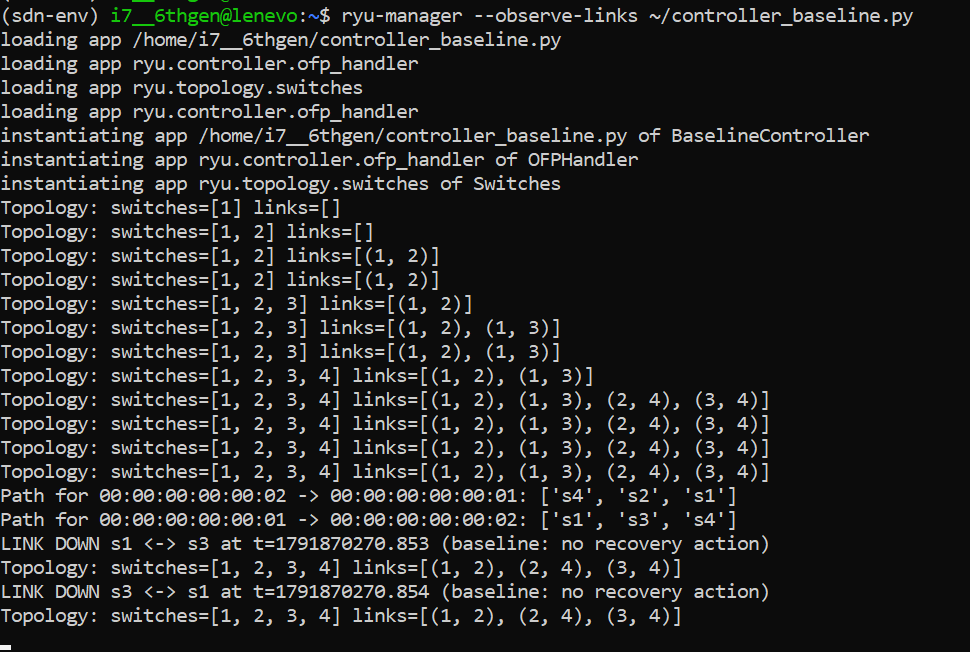
\includegraphics[width=\columnwidth]{figures/topology-discovered.png}
\caption{Topology-discovery evidence for the multipath control workflow.}
\label{fig:topology}
\end{figure}

\begin{figure}[t]
\centering
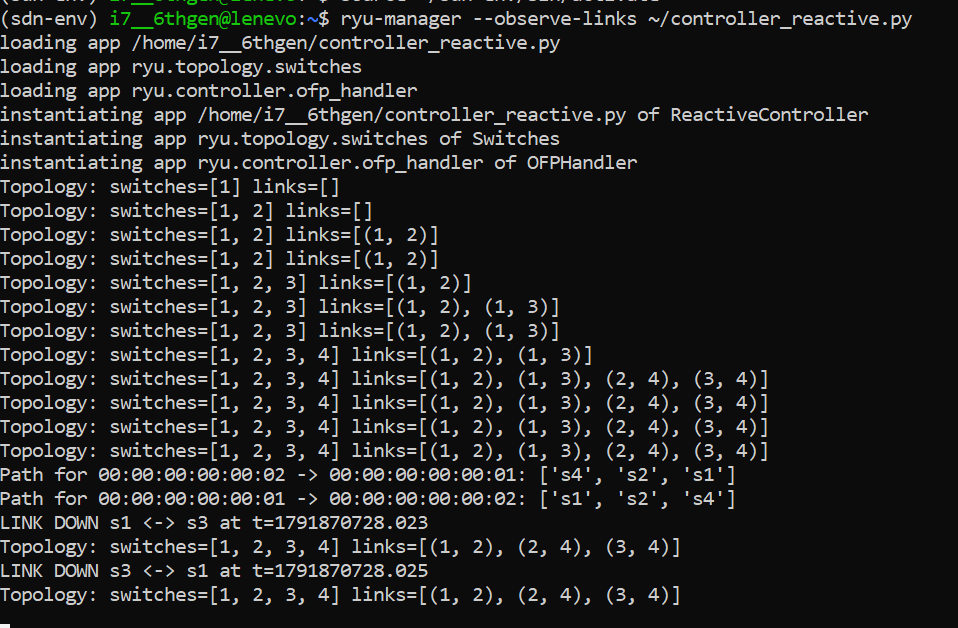
\includegraphics[width=\columnwidth]{figures/reactive-healed-log.png}
\caption{Reactive healing event showing affected-link processing and route
replacement.}
\label{fig:reactive}
\end{figure}

\begin{figure}[t]
\centering
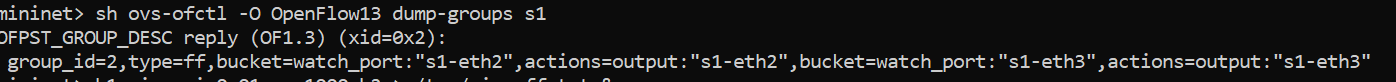
\includegraphics[width=\columnwidth]{figures/ff-group-table.png}
\caption{OpenFlow fast-failover group-table evidence with backup buckets.}
\label{fig:ff}
\end{figure}

\begin{figure}[t]
\centering
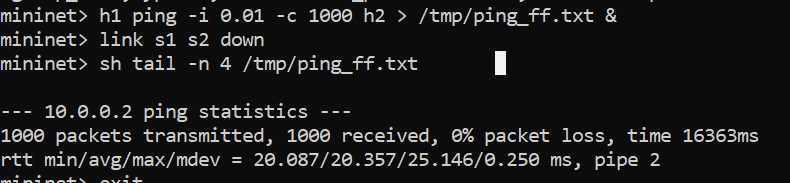
\includegraphics[width=\columnwidth]{figures/ff-ping-result.png}
\caption{Fast-failover traffic result used to inspect service continuity.}
\label{fig:ffping}
\end{figure}

\subsection{Performance analysis}

The results show three distinct performance regimes. Idle and 2 Mbps traffic
remain in a low-latency region. At 4 Mbps, the larger RTT and nonzero loss
indicate queueing or congestion effects. The delay-ramp samples show that an
operational link can cause severe service degradation without packet loss.
Consequently, a self-healing controller should combine port status, utilization,
loss, RTT, and jitter rather than use a single binary link signal.

The baseline, reactive, and fast-failover strategies also expose different
control costs. Baseline has no recovery action and therefore has the lowest
controller-side recovery work. Reactive sends flow deletions and additions
after a topology event. Fast failover installs more state before the failure,
but shifts the primary selection decision into the switch. Adaptive adds
policy evaluation and can select a bounded recovery action from measured
telemetry.

\subsection{Measurement interpretation}

The project records controller processing intervals, traffic counters, and
topology state as separate fields. A controller log event establishes that a
recovery procedure ran. End-to-end transmitted and received counters establish
service behavior. Flow and group-table inspection establishes installed
forwarding state. These evidence types are correlated by controller mode,
topology, experiment identifier, and timestamp.

\section{Discussion}
\label{sec:discussion}

\subsection{Benefits}

The combined platform improves on a single-script SDN demonstration in five
ways. First, controller strategies are interchangeable, allowing a baseline
comparison. Second, topology discovery removes dependence on one hard-coded
port map in the expanded controllers. Third, fast-failover groups provide
switch-local protection. Fourth, telemetry and labelled traffic connect
control actions to service measurements. Fifth, the management API and
dashboard provide persistent operational context instead of isolated terminal
logs.

\subsection{Design trade-offs}

Reactive routing is flexible and can adapt to topologies that change
dynamically, but it requires controller processing after a failure. Fast
failover can switch locally, but it requires preinstalled group state and
careful port ordering. Threshold-based alerts are simple to interpret, but
their accuracy depends on baseline quality and threshold calibration.
SQLite is convenient for a course project and experiment history, while a
high-volume deployment would use a more scalable time-series or relational
backend.

\subsection{Security and deployment}

The management layer is designed for a controlled laboratory environment.
Operational deployment should bind the API to a protected interface, require
authentication and authorization for destructive actions, restrict CORS and
WebSocket origins, protect the worker socket, and execute Mininet operations
with least privilege. These controls are part of the deployment architecture
required for a production-grade SDN platform.

\section{Conclusion}
\label{sec:conclusion}

This paper presented a complete multi-strategy self-healing SDN project. The
system combines a Mininet/Open vSwitch data plane, Ryu/OpenFlow controllers,
NetworkX path computation, telemetry, rule-based alerting, labelled traffic
analysis, a multipath topology, a FastAPI/SQLite management service, and a
React dashboard. Baseline, reactive, fast-failover, and adaptive strategies
provide different points in the recovery design space.

The stored measurements demonstrate the effect of traffic and impairment on
service quality: average RTT increases from 26.80 ms at idle to 30.98 ms
under 2 Mbps load, 70.83 ms under 4 Mbps load, and 157.00 ms during delay
ramp. The alert results show that baseline-relative traffic analysis detects
large host-rate deviations. The mathematical formulation and algorithms
provide a reproducible basis for path selection, telemetry derivation,
recovery, and performance comparison.

The completed platform provides a strong foundation for future experiments
with larger topologies, service-level objectives, controller selection
policies, and secure deployment. Its architecture makes those extensions
possible without changing the fundamental telemetry, persistence, or
dashboard contracts.

\appendices
\section{Implementation Traceability}
\label{app:traceability}

Table~\ref{tab:files} maps the report components to the implemented project
files. This mapping provides direct traceability from each research claim to
the corresponding source module.

\begin{table*}[t]
\centering
\caption{Implementation-to-report traceability}
\label{tab:files}
\begin{tabular}{p{0.20\textwidth}p{0.30\textwidth}p{0.39\textwidth}}
\toprule
Subsystem & Primary files & Reported responsibility\\
\midrule
Original topology & \texttt{topology.py} & Four-switch diamond, fixed hosts, TCLinks, static ARP\\
Original routing & \texttt{controller.py} & Port-status detection, graph update, shortest-path recovery\\
Telemetry & \texttt{telemetry.py} & OpenFlow counter polling and CSV rate derivation\\
Alerts & \texttt{alerts.py} & Congestion windows, host baselines, anomaly alerts\\
Data generation & \texttt{generate\_data.py} & Labelled RTT, jitter, and loss scenarios\\
Controller framework & \texttt{controllers/common.py} & Datapath registry, topology discovery, packet handling\\
Baseline strategy & \texttt{controllers/baseline.py} & Shortest-path forwarding reference\\
Reactive strategy & \texttt{controllers/reactive.py} & Affected-flow deletion and alternate-path installation\\
Fast failover & \texttt{controllers/fast\_failover.py} & Type-FF groups and watch-port buckets\\
Adaptive strategy & \texttt{controllers/adaptive.py} & Backend-owned adaptive decision boundary\\
Mesh topology & \texttt{topo\_multipath\_mesh.py} & Nine-switch redundant topology\\
Management backend & \texttt{backend/main.py} & Health, topology, telemetry, alert, event, and experiment APIs\\
Persistence & \texttt{backend/db.py} & SQLite experiments, events, and recovery records\\
Dashboard & \texttt{frontend/src/} & React health, telemetry, topology, and experiment views\\
\bottomrule
\end{tabular}
\end{table*}

\section{API and Data Contracts}
\label{app:api}

The management layer uses JSON request and response objects. The health
contract contains \texttt{status}, \texttt{database}, and
\texttt{telemetry\_file}. A telemetry response contains a bounded \texttt{rows}
array and a \texttt{summary} object with \texttt{samples},
\texttt{max\_utilization\_pct}, and \texttt{average\_utilization\_pct}.
An experiment request contains a controller mode, topology name, and optional
failure-link key. A persisted experiment contains an identifier, status,
timestamps, and a summary object.

\begin{table}[t]
\centering
\caption{Management API contract}
\label{tab:api}
\begin{tabular}{p{0.25\columnwidth}p{0.18\columnwidth}p{0.43\columnwidth}}
\toprule
Endpoint & Method & Function\\
\midrule
\texttt{/api/health} & GET & Service and telemetry status\\
\texttt{/api/topologies} & GET & Complete topology catalog\\
\texttt{/api/topology/\{name\}} & GET & Nodes and links for one topology\\
\texttt{/api/telemetry} & GET & Recent rows and utilization summary\\
\texttt{/api/alerts} & GET & Recent alert-log lines\\
\texttt{/api/events} & GET & Persisted event records\\
\texttt{/api/experiments} & GET & Experiment history\\
\texttt{/api/experiments} & POST & Create an experiment plan\\
\bottomrule
\end{tabular}
\end{table}

\section{Reproducibility Protocol}
\label{app:reproducibility}

The following protocol defines a repeatable course-project experiment:
\begin{enumerate}
\item Create the selected topology with OpenFlow 1.3 switches and 10 Mbps,
  5 ms switch-to-switch links.
\item Start exactly one selected Ryu controller strategy and confirm the
  datapaths and topology links in its log.
\item Start telemetry collection and confirm that the CSV header and first
  counter-derived rows are present.
\item Start a controlled ICMP or iperf3 traffic window and record its start
  timestamp, source, destination, packet count, and interval.
\item Inject one hard link failure or one soft impairment at a recorded
  timestamp.
\item Collect controller events, telemetry rows, alert events, flow/group
  state, transmitted packets, received packets, RTT, and jitter.
\item Restore the link or impairment, close the traffic window, and persist
  the experiment summary.
\item Repeat the same scenario for each controller mode and topology.
\item Calculate means, loss, relative RTT change, recovery score, and
  confidence intervals from the resulting experiment records.
\end{enumerate}

\begin{table}[t]
\centering
\caption{Recommended experiment record}
\label{tab:record}
\begin{tabular}{p{0.42\columnwidth}p{0.42\columnwidth}}
\toprule
Field & Description\\
\midrule
Experiment ID & Unique management-layer identifier\\
Controller and topology & Selected comparison factors\\
Failure link & Affected inter-switch edge\\
Traffic window & Packet count, interval, source, destination\\
Control event & Detection, route change, and processing timestamps\\
Service evidence & Tx, Rx, loss, RTT, jitter, reachability\\
Dataplane evidence & Flow entries, groups, ports, and path state\\
Final status & Completed, recovered, degraded, or failed\\
\bottomrule
\end{tabular}
\end{table}

\section{Data Dictionary}
\label{app:data}

\begin{table*}[t]
\centering
\caption{Telemetry and labelled-data fields}
\label{tab:data}
\begin{tabular}{p{0.18\textwidth}p{0.23\textwidth}p{0.42\textwidth}}
\toprule
Field & Unit & Meaning\\
\midrule
\texttt{timestamp} & Unix seconds & Time of the observation\\
\texttt{switch} & datapath ID & OpenFlow switch identifier\\
\texttt{port} & port number & Switch port represented by the row\\
\texttt{link} & label & Inter-switch label or host-facing label\\
\texttt{tx\_mbps}, \texttt{rx\_mbps} & Mbps & Counter-derived data rates\\
\texttt{tx\_pps}, \texttt{rx\_pps} & packets/s & Counter-derived packet rates\\
\texttt{utilization\_pct} & percent & Maximum direction rate divided by capacity\\
\texttt{drops}, \texttt{errors} & packets/counters & Counter deltas over the interval\\
\texttt{scenario} & category & Traffic or impairment condition\\
\texttt{label} & class & Scenario label used by the data workflow\\
\texttt{rtt\_ms} & ms & End-to-end round-trip latency\\
\texttt{jitter\_ms} & ms & Variation in RTT samples\\
\texttt{loss\_pct} & percent & End-to-end packet loss\\
\bottomrule
\end{tabular}
\end{table*}

\section{Extended Results Interpretation}
\label{app:interpretation}

The labelled dataset contains 117 samples across four recorded scenarios:
32 idle samples, 25 samples at 2 Mbps load, 24 samples at 4 Mbps load, and
36 delay-ramp samples. The average RTT rises monotonically across the
increasing-load and delay conditions. The 4 Mbps case contributes the observed
0.83 percent average loss, while the delay-ramp case shows a large RTT
increase with zero average loss. This distinction demonstrates the value of
combining reachability, loss, RTT, jitter, and utilization in a recovery
decision.

The alert records contain two H1 anomaly events. The first records 3.0 Mbps
against a near-zero normal rate and a 30.1 times deviation. The second records
2.2 Mbps against a 0.1 Mbps normal rate and a 20.0 times deviation. The
cooldown and baseline logic prevent every telemetry row from becoming a
duplicate event.

\section{Project Deliverables}
\label{app:deliverables}

The final project package contains:
\begin{itemize}
\item the original four-switch prototype and stored data;
\item reusable controller strategy modules;
\item the nine-switch multipath topology;
\item FastAPI backend and SQLite persistence;
\item React/TypeScript dashboard source;
\item IEEE paper source and bibliography;
\item HTML browser preview with print support;
\item topology, recovery, fast-failover, ping, and labelled-data figures.
\end{itemize}

\begin{thebibliography}{00}

\bibitem{mckeown}
N. McKeown \emph{et al.}, ``OpenFlow: Enabling innovation in campus networks,''
\emph{ACM SIGCOMM Computer Communication Review}, vol. 38, no. 2,
pp. 69--74, Apr. 2008.

\bibitem{lantz2010}
B. Lantz, B. Heller, and N. McKeown, ``A network in a laptop: Rapid prototyping
for software-defined networks,'' in \emph{Proc. ACM HotNets}, 2010.

\bibitem{openflow13}
Open Networking Foundation, \emph{OpenFlow Switch Specification Version 1.3.5},
Technical Specification, 2015.

\bibitem{ryu}
Ryu Project, ``Ryu SDN framework.'' [Online]. Available:
\url{https://ryu-sdn.org/}

\bibitem{networkx}
NetworkX Developers, ``NetworkX: Network analysis in Python.'' [Online].
Available: \url{https://networkx.org/}

\bibitem{ovs}
B. Pfaff \emph{et al.}, ``The design and implementation of Open vSwitch,''
in \emph{Proc. USENIX NSDI}, 2015, pp. 117--130.

\bibitem{mininet}
Mininet Developers, ``Mininet: An instant virtual network.'' [Online].
Available: \url{https://mininet.org/}

\end{thebibliography}

\end{document}
